\section{Geometry in 2D}
Be careful of rounding errors. Define $E$ in function of the problem.
\lstinline|Double.parseDouble| is a lot slower than \lstinline|Integer.parseInt|.
\begin{lstlisting}
boolean eq(double a,double b){return Math.abs(a - b) <= E;}
boolean le(double a,double b){return a < b - E;}
boolean leq(double a,double b){return a <= b + E;}
\end{lstlisting}
\subsection{Areas}
Let $D$ be a simple closed curve and $C$ its boundary. For any
function $F(x, y) = (F_1(x, y), F_2(x, y))$ such that $\partial F_2 \slash \partial x - \partial F_1 \slash \partial y =  1$
we have $\textit{area}(D) = \int_C F(s) ds$. Recall that $\int_C F(s) ds = \int_a^b F(r(t)) \cdot r'(t) dt$ where $r : [a, b] \rightarrow C$
is a parametrization of $C$. Usual parametrization of a line segment $(x_1, y_1)$ to $(x_2, y_2)$: $r(t) = (x_1 + t(x_2 - x_1), y_1 + t(y_2 - y_1)), t \in [0, 1]$. Usual parametrization
of a circle arc $\theta_1$ to $\theta_2$: $r(t) = (R \cos(t), R \sin(t)), t \in [\theta_1, \theta_2]$.

\textbf{Example:} Choose for instance $F(x, y) = (0, x)$ we have $\partial F_2 \slash \partial x - \partial F_1 \slash \partial y = 
\partial x \slash \partial x - \partial 0 \slash \partial y = 1 - 0 = 1$. For the segment we have:
$$
F(r(t)) = (x_1 + t(x_2 - x_1), y_1 + t(y_2 - y_1)) = (0, x_1 + t(x_2 - x_1))
$$
$$
r'(t) = (x_2 - x_1, y_2 - y_1)
$$
The contribution of a line segment is:
\footnotesize
\begin{align*}
\int_0^1 F(r(t)) r'(t) dt & = \int_0^1 (0, x_1 + t(x_2 - x_1)) \cdot (x_2 - x_1, y_2 - y_1) \\
& = \int_0^1 t (x_2 - x_1) (y_2 - y_1) = \frac{(x_2 - x_1) (y_2 - y_1)}{2}
\end{align*}
\normalsize
For the circle arc we have:
$$
F(r(t)) = (R \cos(t), R \sin(t)) = (0, R \cos(t))
$$
$$
r'(t) = (-R \sin(t), R \cos(t))
$$
The contribution of a circle arc is:
\footnotesize
\begin{align*}
\int_{\theta_1}^{\theta_2} F(r(t)) r'(t) dt & = \int_{\theta_1}^{\theta_2} (0, R \cos(t)) \cdot (-R \sin(t), R \cos(t)) \\
& = \int_{\theta_1}^{\theta_2} R^2 \cos^2(t) = \frac{R^2}{2} \left( t + sin(t) cos(t) \right) \Big|_{\theta_1}^{\theta_2}  \\
& = \frac{R^2}{2} \left( \theta_2 + sin(\theta_2) cos(\theta_2) - \theta1 - sin(\theta_1) cos(\theta_1) \right)
\end{align*}
\begin{center}
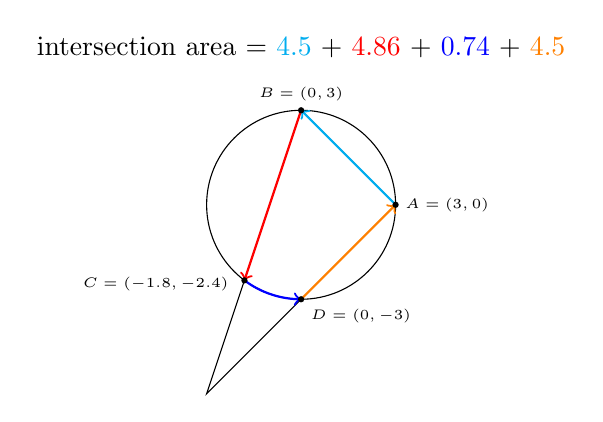
\begin{tikzpicture}[scale = 0.4]
\draw (0, 3) -- (3, 0) -- (-3, -6) -- (0, 3);
\draw (0, 0) circle (3);

\draw[->, cyan, thick] (3, 0) -- (0, 3);
\draw[->, red, thick] (0, 3) -- (-1.8, -2.4);
\draw[->, orange, thick] (0, -3) -- (3, 0);
\draw[->, blue,thick,domain=233:270] plot ({3 * cos(\x)}, {3 * sin(\x)});

\node[anchor = south] at (0, 3) {\tiny $B = (0, 3)$};
\node[anchor = west] at (3, 0) {\tiny $A = (3, 0)$};
\node[anchor = north east] at (-2, -2) {\tiny $C = (-1.8, -2.4)$};
\node[anchor = north west] at (0, -3) {\tiny $D = (0, -3)$};
\fill (0, 3) circle (0.1);
\fill (0, -3) circle (0.1);
\fill (3, 0) circle (0.1);
\fill (-1.8, -2.4) circle (0.1);

\node at (0, 5) {intersection area = {\color{cyan}4.5} +  {\color{red}4.86} +  {\color{blue}0.74} +  {\color{orange}4.5}};
\end{tikzpicture}
\end{center}

\subsection{Vectors}
\subsubsection{Rotation around (0,0)}
$(x, y) \leftrightarrow x + y i$\\
$\rho e^{i\theta} = \rho \cos(\theta) + i \rho \sin(\theta)$\\

$(x, y)$ rotated by $\alpha$ is
$(\cos(\alpha) x - \sin(\alpha) y, \sin(\alpha)  x + \cos(\alpha) y)$
\subsection{Points}
\begin{lstlisting}
class Point implements Comparable<Point>
{
  double x, y;
  public int compareTo(Point o) { //xcomp
    if(a.x < b.x) return -1;
    if(a.x > b.x) return 1;
    if(a.y < b.y) return -1;
    if(a.y > b.y) return 1;
    return 0;
  }
}

class yComp implements Comparator<Point> {
  public int compare(Point p, Point q) {
    if(p.y == q.y) {return Double.compare(p.x, q.x);}
    return Double.compare(p.y, q.y);
  }
}
\end{lstlisting}
\subsubsection{Point in box}
\begin{lstlisting}
boolean inBox(Point p1, Point p2, Point p) {
  return Math.min(p1.x, p2.x) <= p.x && p.x <= Math.max(p1.x, p2.x) &&			           
         Math.min(p1.y, p2.y) <= p.y && p.y <= Math.max(p1.y, p2.y);
}
\end{lstlisting}
\subsubsection{Polar sort}
\begin{lstlisting}
LinkedList<Point> sortPolar(Point[] P, Point o)
{
  LinkedList<Point> above = new LinkedList<Point>();
  LinkedList<Point> samePos = new LinkedList<Point>();
  LinkedList<Point> sameNeg = new LinkedList<Point>();
  LinkedList<Point> bellow = new LinkedList<Point>();
  for(Point p : P)
  {
    if(p.y > o.y)
      above.add(p);
    else if(p.y < o.y)
      bellow.add(p);
    else
    {
      if(p.x < o.x)
        sameNeg.add(p);
      else
        samePos.add(p);

    }
  }
  PolarComp comp = new PolarComp(o);    
  Collections.sort(samePos, comp);
  Collections.sort(sameNeg, comp);
  Collections.sort(above, comp);
  Collections.sort(bellow, comp);
  LinkedList<Point> sorted = new LinkedList<Point>();
  for(Point p : samePos) sorted.add(p);
  for(Point p : above) sorted.add(p);
  for(Point p : sameNeg) sorted.add(p);
  for(Point p : bellow) sorted.add(p);
  return sorted;
}

class PolarCmp implements Comparator<Point> {
  static Point orig = new Point(0, 0);
  public int compare(Point p, Point q) {
    double o = orient(orig, p, q);
    if(o == 0) {
      if(p.x * p.x + p.y * p.y > q.x * q.x + q.y * q.y)
        return 1;
      return -1;
    }
    return -(int)Math.signum(o);
  }
}
\end{lstlisting}
\subsubsection{Closest pair of points}
\begin{lstlisting}
double closestPair(Point[] points) {
  if(points.length == 1) {return Double.POSITIVE_INFINITY;}
  Arrays.sort(points, new xComp());
  double min = dist(points[0], points[1]);
  // keep track of the leftmost point
  int leftmost = 0;
  TreeSet<Point> candidates = new TreeSet<Point>(new yComp());
  candidates.add(points[0]);
  candidates.add(points[1]);
  for(int i = 2; i < points.length; i++) {
    Point cur = points[i];
    // eliminate points s.t cur.x - x > min 
    while(cur.x - points[leftmost].x > min) {
      candidates.remove(points[leftmost]);
      leftmost++;
    }
    Point low = new Point(0, cur.y - min);
    Point high = new Point(0, cur.y + min);
    // check all points in the rectangle
    for(Point point : candidates.subSet(low, high))
      min = Math.min(min, dist(cur, point));
    candidates.add(cur);
  }
  return min;
}
\end{lstlisting}
\subsubsection{Orientation}
$$
orient(p, q, r) = 
\begin{vmatrix}
1 & p_x & p_y \\
1 & q_x & q_y \\
1 & r_x & r_y
\end{vmatrix}
$$

$$
orient(p, q, r) \left\{
\begin{array}{l l l}
= 0 \quad & \text{$p, q, r$ are collinear} \\
< 0 \quad & \text{$p$ -> $q$ -> $r$ is clockwise} \\
> 0 \quad & \text{$p$ -> $q$ -> $r$ is counterclockwise}
\end{array} \right.
$$

$$
|orient(p, q, r)| = 2 \cdot area \ \triangle(p, q, r)
$$

\begin{lstlisting}
double orient(Point p, Point q, Point r) {
  return q.x * r.y - r.x * q.y - p.x * (r.y - q.y) + p.y * (r.x - q.x);
}
\end{lstlisting}
\subsubsection{Angle visibility}
$x$ lies strictly inside the angle formed by $p, q, r$ iff
\begin{align*}
sgn(orient(p, q, x)) & = sgn(orient(p, x, r)) \\
sgn(orient(p, r, x)) & = sgn(orient(p, x, q)) \\
\end{align*}
To allow it to lie on the border simply check if $$sgn(orient(p, q, x)) = 0 \text{ or } sgn(orient(p, r, x)) = 0$$
\subsubsection{Fixed radius neighbors (1D)}
\begin{lstlisting}
List<Double[]> findPairs1D(double[] x, double r) {
  HashMap<Integer, List<Double>> H = new HashMap<Integer, List<Double>>();
  // fill buckets
  for(int i = 0; i < x.length; i++) {
    int b = (int)(x[i] / r);
    if(H.containsKey(b)) {
      H.get(b).add(x[i]);
    } else {
      List<Double> L = new ArrayList<Double>();
      L.add(x[i]);
      H.put(b, L);				
    }
  }
  // find pairs in consecutive buckets
  List<Double[]> pairs = new LinkedList<Double[]>(); 
  for(int i = 0; i < x.length; i++) {
    int b = (int)(x[i] / r);
    List<Double> bucket = H.get(b + 1);
    if(bucket != null)
      for(double y : bucket)
        if(y - x[i] <= r)
          pairs.add(new Double[] {x[i], y});
  }
  // add points in buckets
  for(List<Double> bucket : H.values())
    for(int i = 0; i < bucket.size(); i++)
      for(int j = i + 1; j < bucket.size(); j++)
        pairs.add(new Double[] {bucket.get(i), bucket.get(j)});
  return pairs;
}
\end{lstlisting}
\subsubsection{Fixed radius neighbors (2D)}
\begin{lstlisting}
List<Point[]> findPairs2D(Point[] points, double r) {
  HashMap<Integer, List<Point>> H = new HashMap<Integer, List<Point>>();
  // fill buckets
  for(int i = 0; i < points.length; i++) {
    int bx = (int)(points[i].x / r);
    int by = (int)(points[i].y / r);
    int key = 33 * bx + by;
    if(H.containsKey(key)) {
      H.get(key).add(points[i]);
    } else {
      List<Point> L = new ArrayList<Point>();
      L.add(points[i]);
      H.put(key, L);				
    }
  }
  // find pairs in adjacent buckets
  List<Point[]> pairs = new LinkedList<Point[]>();
  int[][] dir = new int[][] {new int[] {1,0}, new int[] {0,1}, new int[] {1,1}};
  for(int i = 0; i < points.length; i++) {
    int bx = (int)(points[i].x / r);
    int by = (int)(points[i].y / r);
    for(int[] d : dir) {
      List<Point> bucket = H.get(33 * (bx + d[0]) + (by + d[1]));
      if(bucket != null)
        for(Point y : bucket)
          if(sqDist(points[i], y) <= r * r)
            pairs.add(new Point[] {points[i], y});					
    }
  }
  // add points in buckets
  for(List<Point> bucket : H.values())
    for(int i = 0; i < bucket.size(); i++)
      for(int j = i + 1; j < bucket.size(); j++)
        if(sqDist(bucket.get(i), bucket.get(j)) <= r * r)			
          pairs.add(new Point[] {bucket.get(i), bucket.get(j)});
  return pairs;
}
\end{lstlisting}

\subsection{Lines}
General equation:$Ax + By = C$. The line through $(x_1, y_1), (x_2, y_2)$ is given by: $A = y_2 - y_1$, $B = x_1 - x_2$, $C = A x_1 + B y_1$.
\subsubsection{Intersections}
Intersection exists there is a solution for $A_1 x + B_1 y = C_1$ and $A_2 x + B_2 y = C_2$. This happens if and only if $$d := \det \begin{pmatrix}
A_1 & B_1 \\
A_2 & B_2 \\
\end{pmatrix} \neq 0$$
Intersection is given by
$$\begin{pmatrix}
x\\
y
\end{pmatrix} = 
\begin{pmatrix}
A_1 & B_1 \\
A_2 & B_2 \\
\end{pmatrix}^{-1} 
\begin{pmatrix}
C_1 \\
C_2
\end{pmatrix}
=
\frac{1}{d}
\begin{pmatrix}
B_2 & -B_1 \\
-A_2 & A_1 \\
\end{pmatrix} 
\begin{pmatrix}
C_1 \\
C_2
\end{pmatrix}
$$
\subsubsection{Perpendicular line}
The lines perpendicular to $Ax + By = C$ are
$$-Bx + Ay = D \quad \text{for $D \in \mathbb{R}$}$$
If we want the one that goes through $(x_0, y_0)$ set
$$D = - B x_0 + A y_0$$
\subsubsection{Orthogonal Symmetry}
For a line, find $X'$, the point which is the orthogonal symmetry of $X$ on line $a$. \\
Computes the perpendicular of the given line that goes through $X$. Compute intersection $Y$. $X' = Y - (X - Y)$.
\subsection{Segments}
\subsubsection{Intersection}
\begin{itemize}
\item Treat segments as lines.
\item If $d \neq 0$, compute line intersection $(x, y)$.
\item Segments intersect iff
\begin{align*}
\min(x_1, x_2) \leq & \ x \leq \max(x_1, x_2) \\
\min(y_1, y_2) \leq & \ y \leq \max(y_1, y_2)
\end{align*}
\end{itemize}
\begin{lstlisting}
boolean intersects(Point p1, Point p2, Point p3, Point p4) {
  double o1 = orient(p1, p2, p3);
  double o2 = orient(p1, p2, p4);
  double o3 = orient(p3, p4, p1);
  double o4 = orient(p3, p4, p2);
  // check first condition of the lemma
  if(o1 * o2 < 0 && o3 * o4 < 0) return true;
  // check seconds condition of the lemma
  if(o1 == 0 && inBox(p1, p2, p3)) return true;
  if(o2 == 0 && inBox(p1, p2, p4)) return true;
  if(o3 == 0 && inBox(p3, p4, p1)) return true;
  if(o4 == 0 && inBox(p3, p4, p2)) return true;
  return false;
}
\end{lstlisting}
\subsubsection{Intersections problem}
Given a lot of segments, return true if it exists a pair that intersects.
\begin{lstlisting}
boolean segmentIntersection(Segment[] S) {
  Event[] events = new Event[2 * S.length];
  // create event points
  for(int i = 0, j = 0; i < S.length; i++) {
    events[j++] = new Event(S[i].l.x, true, S[i]);
    events[j++] = new Event(S[i].r.x, false, S[i]);
  }
  Arrays.sort(events);
  SegmentCmp cmp = new SegmentCmp();
  TreeSet<Segment> T = new TreeSet<Segment>(cmp);
  // sweep line
  for(Event event : events) {
    Segment s = event.s;
    cmp.x = event.x;
    if(event.isLeft) {
      // new segment found. check if it intersects one of its neighbors
      T.add(s);
      Segment above = T.higher(s);
      Segment bellow = T.lower(s);
      if((above != null && intersects(above, s)) || 
         (bellow != null && intersects(bellow, s)))
        return true;
    } else {
      // end of segment. check if its neighbors intersect
      Segment above = T.higher(s);
      Segment bellow = T.lower(s);
      if(above != null && bellow != null && intersects(above, bellow))
        return true;
      T.remove(s);
    }
  }
  return false;
}

class Event implements Comparable<Event> {
  double x;
  boolean isLeft;
  Segment s;
  public Event(double x, boolean isLeft, Segment s) {
    this.x = x;
    this.isLeft = isLeft;
    this.s = s;
  }
  public int compareTo(Event other) {
    int cmp = Double.compare(x, other.x);
    // ensure that left comes before right
    if(cmp == 0) return isLeft? -1 : 1;
    return cmp;
  }
  public String toString() {
    return x + " " + isLeft;
  }
}

class SegmentCmp implements Comparator<Segment> {
  double x;
  public int compare(Segment s1, Segment s2) {
    // compute A,B,C from eq Ax + by = C for each segment
    double A1 = s1.r.y - s1.l.y;
    double B1 = s1.l.x - s1.r.x;
    double C1 = A1 * s1.l.x + B1 * s1.l.y;

    double A2 = s2.r.y - s2.l.y;
    double B2 = s2.l.x - s2.r.x;
    double C2 = A2 * s2.l.x + B2 * s2.l.y;

    // no divisions =)
    double t1 = B2 * (C1 - A1 * x);
    double t2 = B1 * (C2 - A2 * x);
    if(t1 == t2) {
      return s1 == s2? 0 : -1;
    } else if(B1 * B2 > 0) {
      return Double.compare(t1, t2);
    } else {
      return Double.compare(t2, t1);
    }
  }
}
\end{lstlisting}
\subsection{Circles}
\subsubsection{Circles from 3 points}
\begin{itemize}
\item 3 non collinear points define a unique circle.
\item Center is intersection of bisectors of $XY$ and $YZ$. 
\end{itemize}
\subsubsection{Circle-line intersection}

\begin{center}
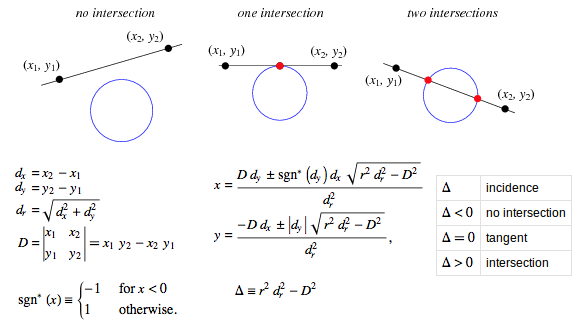
\includegraphics[scale=0.45]{Geometrie/circleLine.png}
\end{center}

\subsubsection{Circle-circle or circle-point tangents}
\newcommand{\acos}{\mbox{acos}}
Find lines tangent to both circles $(C_1,r_1)$ and $(C_2,r_2)$. Let $d = |C_1C_2|$.
\begin{itemize}
\item{\bf Inner tangents:} Condition: $r_1+r_2 \leq d$ (if equal, only one). Let $\alpha = \acos(\frac{r_1+r_2}{d})$, then the tangency two points $T$ on either circle are such that $\widehat{C_2C_1T}=\alpha$ and $\widehat{C_1C_2T}=\alpha$ respectively.
\item{\bf Outer tangents:} Condition: $|r_1-r_2| \leq d$ (if equal, only one). Same, but with $\widehat{C_2C_1T}=\acos(\frac{r_1-r_2}{d})$ and $\widehat{C_1C_2T}=\acos(\frac{r_2-r_1}{d})$.
\end{itemize}
For circle-point tangents, set $r_2=0$ on inner tangents.
\subsection{Polygons}
\subsubsection{Triangulation}
A vertex $i$ of a polygon is a ear if the triangle formed by vertices
$i - 1$, $i$ and $i + 1$ is inside the polygon. Every polygon has at
least two ears. Therefore to triangulate we can remove the ears 
until only a triangle remains. Any triangulation has always exactly 
$n - 2$ triangles. Implemented naivelly this gives a $O(n^3)$ algorithm.
Can be implemented in $O(n^2)$. Faster algorithms exists: 
sweep line does it in $O(n \log(n))$ but is it harder.
\begin{lstlisting}
// assumes that pol is in counter-clockwise order
private static boolean ear(Point[] pol, int i) {
  int n = pol.length;
  int j = (i - 1 + n) % n;
  int k = (i + 1 + n) % n;
  // if ccw then points must also be ccw
  if(orient(pol[j], pol[i], pol[k]) < eps) return false;
  for(int m = 0; m < n; m++)
    // inTriangle not in the sheets. checks if pol[m] is inside triangle pol[j]pol[i]pol[k]
    if(m != i && m != j && m !=k && inTriangle(pol[m], pol[j], pol[i], pol[k]))
      return false;
  return true;
}
\end{lstlisting}

\subsubsection{Triangles}
\begin{itemize}
  \item côtés $a,b,c$, angles $A,B,C$, hauteurs $h_A,h_B,h_C$, $s=\frac{a+b+c}{2}$, aire $S$.
  \item Aire: $S=ah_A/2$, $S=ab\sin C/2$, $S=\sqrt{s(s-a)(s-b)(s-c)}$.
  \item Inradius $r=\frac{S}{s}$.
  \item Outradius $2R = \frac{a}{\sin A} = \frac{b}{\sin B} = \frac{c}{\sin C}$.
  \item $rR = \frac{abc}{4s}$.
\end{itemize}
\subsubsection{Check convexity}
\begin{lstlisting}
boolean isConvex(Point[] P) {
  if(P.length < 3) return false;
  double o1 = orient(P[P.length-1], P[0], P[1]);
  for (int i = 0; i < P.length; i++) {
    double o2 = orient(P[i], P[i + 1], P[i + 2]);
    if(o1 * o2  < 0) {
      return false;
    } else if (o2 != 0) {
      o1 = o2;
    }
  }
  return true;
}
\end{lstlisting}
\subsubsection{Winding number}
Number of times a path of points "turn around" another point. (can check if a point is inside a polygon: in this case, winding numbe $!=0$)
\begin{lstlisting}
// assumes p is not on P
double winding(Point[] P, Point p) {
  //make a translation so p = (0, 0)
  for(Point q : P) {
    q.x -= p.x;
    q.y -= p.y;
  }
  double w = 0;
  for(int i = 0; i < P.length - 1; i++) {
    if(P[i].y * P[i + 1].y < 0) {
      // segment crosses the x-axis
      double r = (P[i].y - P[i+1].y) * P[i].x + P[i].y * (P[i+1].x - P[i].x);
      //check for intersection with the positive x-axis
      if((P[i].y - P[i+1].y > 0 && r > 0) || (P[i].y - P[i+1].y < 0 && r < 0)) {
        // segment fully crosses the x-axis
        // - to + add 1, + to - subtract 1
        w += P[i].y < 0? 1 : -1;
      } else if(P[i].y == 0 && P[i].x > 0) {
        // the segment starts at the x-axis
        // 0 to + add 0.5, 0 to - subtract 0.5
        w += P[i+1].y > 0? 0.5 : -0.5;
      } else if(P[i+1].y == 0 && P[i+1].x > 0) {
        // the segment ends at the x-axis
        // - to 0 add 0.5, + to 0 subtract 0.5
        w += P[i].y < 0? 0.5 : -0.5;
      }
    }
  }
  return w;
}
\end{lstlisting}
\subsubsection{Convex Hull}
\begin{lstlisting}
Point[] convexHull(Point[] points) {
  // sort points by increasing x coordinates
  Arrays.sort(points, new xComp());
  // build upper chain
  Point[] upChain = buildChain(points, 1);
  // build lower chain
  Point[] loChain = buildChain(points, -1);
  Point[] hull = new Point[upChain.length + loChain.length - 2];
  int i;
  // build convex hull from upper and lower chain
  for(i = 0; i < upChain.length; i++) {
    hull[i] = upChain[i];
  }
  for(int j = loChain.length - 2; j >= 1; j--) {
    hull[i] = loChain[j]; i++;
  }
  return hull;
}

Point[] buildChain(Point[] points, int sgn) {
  Point[] S = new Point[points.length];
  int k = 0;
  S[k++] = points[0]; // push points[0]
  S[k++] = points[1]; // push points[1]
  // build chain
  for(int i = 2; i < points.length; i++) {
    //double orient = orient(S[k - 2], S[k - 1], points[i]);
    while(k >= 2 && sgn * orient(S[k - 2], S[k - 1], points[i]) >= 0) {
      S[k - 1] = null; // pop
      k--;
    }
    S[k++] = points[i]; // push points[i]
  }
  return Arrays.copyOf(S, k);
}
\end{lstlisting}

\subsection{Interval Tree}

\begin{center}
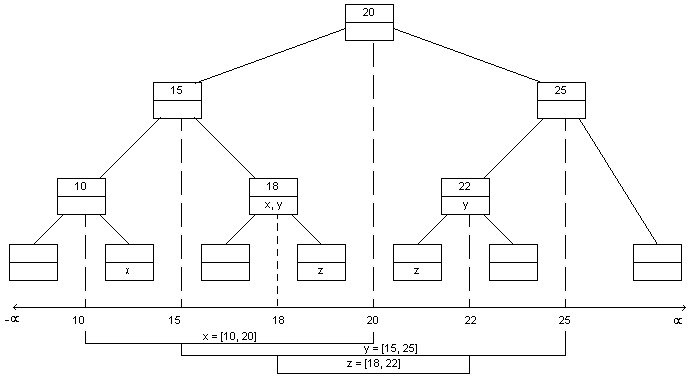
\includegraphics[scale=0.35]{Geometrie/it.png}
\end{center}

\lstinputlisting{Geometrie/intervaltree.java}

\subsection{Area of union of rectangles}

\lstinputlisting{Geometrie/rectangles.java}

%\subsection{C library by Xiao}
%\lstset{language=C}
%{\setmainfont{CODE2000.TTF} % font that supports chinese
%\lstinputlisting{Geometrie/Geometry.h}
%}
%\lstset{language=Java}

\section{Geometry in 3D}
\subsection{Cross product}
With vectors $\vec{V_1}=(a_1, b_1, c_1)$ and $\vec{V_2}=(a_2, b_2, c_2)$:
$$\vec{V_1}\times\vec{V_2}=(b_1c_2-c_1b_2, c_1a_2-a_1c_2, a_1b_2-b_1a_2)$$
\subsection{Equation of a plane}
\subsubsection{with a normal vector and a point}
A plane is defined by a point $(x_0, y_0, z_0)$ and an normal vector $(a, b, c)$.
$$a(x-x_0)+b(y-y_0)+c(z-z_0)=0$$
$$ax+by+cz=ax_0+by_0+cz_0=d$$
\subsubsection{with a point and two vectors in the plane}
A plane is defined by a point $(x_0, y_0, z_0)$ and two vectors $(\alpha_1, \beta_1, \gamma_1)$ and $(\alpha_2, \beta_2, \gamma_2)$. We obtain the parametric equations:
$$x=x_0+t_1\alpha_1+t_2\alpha_2$$
$$y=y_0+t_1\beta_1+t_2\beta_2$$
$$z=z_0+t_1\gamma_1+t_2\gamma_2$$
Or we can find the normal vector of the plane by doing the vector product of the two vectors
\subsubsection{with three points}
Make vectors from these three points and use one of the methods above.
\subsection{Equation of a line}
\subsubsection{With a point and a vector}
A line is defined by a point $(x_0, y_0, z_0)$ and a vector $(a, b, c)$.
$$x=x_0+ta$$
$$y=y_0+tb$$
$$z=z_0+tc$$
\subsubsection{With two points}
$$x=x_1+t(x_2-x_1)$$
$$y=y_1+t(y_2-y_1)$$
$$z=z_1+t(z_2-z_1)$$
\subsection{Distance from a point to a line}
Distance from a point $M_P=(x_p, y_p, z_p)$ to a line defined with a point $M_L=(x_l, y_l, z_l)$ and a vector $\vec{V}=(a, b, c)$ equals to
$$\frac{||\vec{M_LM_P}\times\vec{V}||}{||\vec{V}||}$$
\subsection{Distance from a point to a plane}
The distance to a plane is 0 if a point is in the plane.
$$\frac{|ax_p+by_p+cz_p-d|}{\sqrt{a^2+b^2+c^2}}$$
\subsection{Orthogonal projection of a point on a line}
If $p_p$ is the point, $s$ the direction vector of the line and $p_l$ the base point for the vector, the projection is
$$\frac{(p_p-p_l)\cdot s}{s\cdot s}s+p_l$$
\subsection{Orthogonal projection of a point on a plane}
$$P_p=(x+\lambda a, y+\lambda b, z + \lambda c)$$
$$\lambda = -\frac{ax_p+by_p+cz_p-d}{a^2+b^2+c^2}$$
\subsection{Orthogonal projection of a line on a plane}
Take two points of the line, project them on the plane, recreate the line from the two new points.
\subsection{Finding if a point is in a 3D polygon}
Take any ray in the plane of the polygon, starting from the point you want to check (simply fix one of the coordinate of the point to find the ray); if it intersects an even number number of time with the sides of the polygon, the point is inside it.
\subsection{Intersection of a line and a plane}
Given a plane $ax+by+cz=d$ and a line with parametric equations:
$x=x_0+\alpha t$, $y=y_0+\beta t$, $z=z_0+\gamma t$
The value of $t$ associated with the intersection is
$$t=\frac{d-ax_0-by_0-cz_0}{a\alpha+b\beta+c\gamma}$$
